
\documentclass[a4paper]{article}
\usepackage[text={165mm,245mm}]{geometry}
\usepackage{graphicx}
\usepackage{subfigure}
\usepackage{ctex}
\usepackage{float} 
\usepackage{amsmath}
\usepackage{listings}
\usepackage{xcolor}
\definecolor{mygreen}{rgb}{0,0.6,0}  
\definecolor{mygray}{rgb}{0.5,0.5,0.5}  
\definecolor{mymauve}{rgb}{0.58,0,0.82}  
  
% RISC-V Assembler syntax and style for latex lstlisting package
% 
% These are risc-v commands as per our university (University Augsburg, Germany) guidelines.
%
% Author: Anton Lydike
%
% This code is in the public domain and free of licensing

% language definition
\lstdefinelanguage[RISC-V]{Assembler}
{
  alsoletter={.}, % allow dots in keywords
  alsodigit={0x}, % hex numbers are numbers too!
  morekeywords=[1]{ % instructions
    lb, lh, lw, lbu, lhu,
    sb, sh, sw,
    sll, slli, srl, srli, sra, srai,
    add, addi, sub, lui, auipc,
    xor, xori, or, ori, and, andi,
    slt, slti, sltu, sltiu,
    beq, bne, blt, bge, bltu, bgeu,
    j, jr, jal, jalr, ret,
    scall, break, nop
  },
  morekeywords=[2]{ % sections of our code and other directives
    .align, .ascii, .asciiz, .byte, .data, .double, .extern,
    .float, .globl, .half, .kdata, .ktext, .set, .space, .text, .word
  },
  morekeywords=[3]{ % registers
    zero, ra, sp, gp, tp, s0, fp,
    t0, t1, t2, t3, t4, t5, t6,
    s1, s2, s3, s4, s5, s6, s7, s8, s9, s10, s11,
    a0, a1, a2, a3, a4, a5, a6, a7,
    ft0, ft1, ft2, ft3, ft4, ft5, ft6, ft7,
    fs0, fs1, fs2, fs3, fs4, fs5, fs6, fs7, fs8, fs9, fs10, fs11,
    fa0, fa1, fa2, fa3, fa4, fa5, fa6, fa7
  },
  morecomment=[l]{;},   % mark ; as line comment start
  morecomment=[l]{\#},  % as well as # (even though it is unconventional)
  morestring=[b]",      % mark " as string start/end
  morestring=[b]'       % also mark ' as string start/end
}

\lstset{ %  
  backgroundcolor=\color{white},   % choose the background color; you must add \usepackage{color} or \usepackage{xcolor}  
  basicstyle=\footnotesize,        % the size of the fonts that are used for the code  
  breakatwhitespace=false,         % sets if automatic breaks should only happen at whitespace  
  breaklines=true,                 % sets automatic line breaking  
  captionpos=bl,                    % sets the caption-position to bottom  
  commentstyle=\color{mygreen},    % comment style  
  deletekeywords={...},            % if you want to delete keywords from the given language  
  escapeinside={\%*}{*)},          % if you want to add LaTeX within your code  
  extendedchars=true,              % lets you use non-ASCII characters; for 8-bits encodings only, does not work with UTF-8  
  frame=single,                    % adds a frame around the code  
  keepspaces=true,                 % keeps spaces in text, useful for keeping indentation of code (possibly needs columns=flexible)  
  keywordstyle=\color{blue},       % keyword style  
  %language=Bin,                 % the language of the code  
  morekeywords={*,...},            % if you want to add more keywords to the set  
  numbers=left,                    % where to put the line-numbers; possible values are (none, left, right)  
  numbersep=5pt,                   % how far the line-numbers are from the code  
  numberstyle=\tiny\color{mygray}, % the style that is used for the line-numbers  
  rulecolor=\color{black},         % if not set, the frame-color may be changed on line-breaks within not-black text (e.g. comments (green here))  
  showspaces=false,                % show spaces everywhere adding particular underscores; it overrides 'showstringspaces'  
  showstringspaces=false,          % underline spaces within strings only  
  showtabs=true,                  % show tabs within strings adding particular underscores  
  stepnumber=1,                    % the step between two line-numbers. If it's 1, each line will be numbered  
  stringstyle=\color{orange},     % string literal style  
  tabsize=2,                       % sets default tabsize to 2 spaces  
  %title=myPython.py                   % show the filename of files included with \lstinputlisting; also try caption instead of title  
}  
\title{\heiti 
CODH - 汇编程序设计 \hspace{0.3cm}实验报告}
\author{院系: \kaishu\underline{}\hspace{1.5cm}姓名: \kaishu \underline{}\hspace{1.5cm}学号: \kaishu \underline{}\hspace{1.5cm}}
\begin{document}
\maketitle

\section{实验目的}
\begin{itemize}
    \item 理解RISC-V常用32位整数指令功能
    \item 掌握RISC-V简单汇编程序设计,以及下载测试数据 (COE文件) 的生成方法
    \item 熟悉RISC-V汇编程序仿真运行环境和调试基本方法
    
    
    
\end{itemize}

\section{实验环境}
\begin{itemize}
  \item macOS 13.0
  \item Rars1\_5.jar (Riscv Assembler and Runtime Simulator)
\end{itemize}
\section{实验内容}
\subsection{设计汇编程序,自动测试以下指令功能}
\begin{itemize}
  \item add, addi, sub, auipc, lui
  \item and, or, xor
  \item slli, srli, srai
  \item lw, sw
  \item beq, blt, bltu, jal, jalr
  
  
\end{itemize}

\subsection{设计汇编程序,实现可变长数组排序}
\begin{itemize}
    \item 数据结构:数组大小,数据元素,
    \item 数据类型:大小和元素均为32位无符号数
    \item 排序算法:算法不限,升序或降序排序
    
  \end{itemize}
  
之后将其与串行调试单元模块(SDU\_DM)整合后,下载至FPGA中测试。

\section{逻辑设计 / 核心代码}
\subsection{设计汇编程序,自动测试以下指令功能}
\subsubsection{逻辑设计}
这里完成了两种测试方式,一种是在测试某一条指令时默认其余指令都可用,通过载入寄存器、执行指令、比较结果并输出三步来完成指令的测试。这里针对18条指令都构建了对应的测试子程序。

另一种方式是从零开始,先检测不需要任何其他指令的beq指令,再以此为基础逐渐添加其他指令的测试,每条指令的测试只可使用之前已经测试完成的指令。
对于测试结果的表示使用了将寄存器的相应位置为1,并且陷入相应的死循环以保存结果显示,这里可能需要用到未经测试的指令(slli)。
\subsubsection{核心代码1}
\begin{lstlisting}[language={[RISC-V]Assembler},title={test.asm}] 
test_add:
    la a1, str_add
    lw a2, arg0
    lw a3, arg1
    lw a4, ans_add
    add a5, a2, a3
    la a0, str_pass
    beq a4, a5, add_pass
    la a0, str_fail
add_pass:
    ret
\end{lstlisting}

\subsubsection{核心代码2}
\begin{lstlisting}[language={[RISC-V]Assembler},title={test1.asm}] 
main:
    addi a6, zero, 1
jal_test:
    jal beq_test
    slli a6, a6, 1
    jal wrong

beq_test:
    beq zero, zero, lw_test
    slli a6, a6, 2
    jal wrong

lw_test:
    lw a0, arg0
    lw a1, arg1
    beq a0, a1, sw_test
    slli a6, a6, 3
    jal wrong

    ...
    \end{lstlisting}

\subsubsection{代码运行}
使用Rars1\_5.jar仿真运行,可以看到两份代码都测试结果正确。
第一种测试:

\begin{figure}[H]
    \centering
    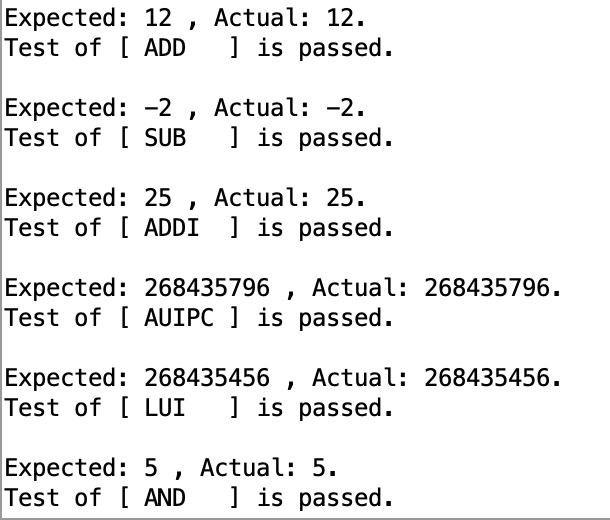
\includegraphics[width=0.8\textwidth]{test.png}
    \caption{test.asm 运行结果}
    \label{fig:test}
  \end{figure}

第二种测试:通过断点可以看到最终陷入表示正确的死循环,且寄存器a6说明运行结果正确。
\begin{figure}[H]
    \centering
    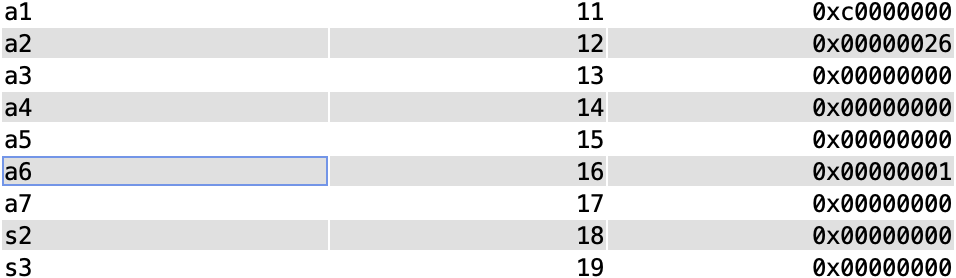
\includegraphics[width=0.8\textwidth]{test1.png}
    \caption{test1.asm 运行结果}
    \label{fig:test1}
  \end{figure}

\subsection{设计汇编程序,实现可变长数组排序}
\subsubsection{逻辑设计}
依然采用冒泡排序,先用高级语言写出后参照结构更改为汇编语言:
\begin{lstlisting}[language={[ANSI]c},title={sort.c}]
    for (int i = 1; i <= n - 1; i++)
        for (int j = 1; j <= n - i + 1; j++)
        if(M[j] > M[j+1]) 
            { swap(M[j], M[j+1]); }
\end{lstlisting}

由此可以写出以下汇编代码,注意循环变量变化方向以及步长有所不同,这是为了匹配RISC-V的地址格式(按字存储):
\subsubsection{核心代码}

\begin{lstlisting}[language={[RISC-V]Assembler},title={srt.asm}]
sort:
    mv t0, a1
    slli t0, t0, 0x2
    addi t6, zero, 0x8
outer_loop:
    addi t0, t0, -0x4
    addi t1, zero, 0
inner_loop: 
    add t2, a0, t1
    addi t1, t1, 0x4
    lw t3, 0(t2)
    lw t4, 0x4(t2)
    blt t3, t4, inner_loop_end
    sw t4, 0(t2)
    sw t3, 0x4(t2)
inner_loop_end:
    blt t1, t0, inner_loop
    bge t0, t6, outer_loop
    ret
\end{lstlisting}
\subsubsection{代码运行} 
使用.data初始化数据段为 x10, xf, xe, xd, xc, xb, xa, x9, x8, x7, x6, x5, x4, x3, x2, x1, x0.
然后在主函数部分,先输出数组内容、进行排序、再输出排序后的数组内容,结果如下:

\begin{figure}[H]
    \centering
    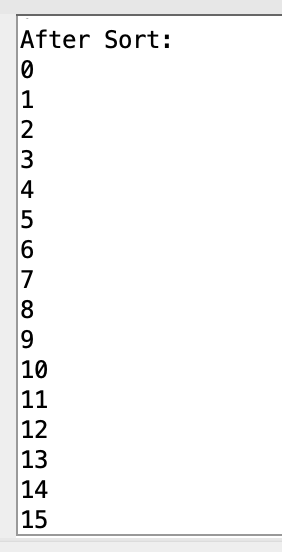
\includegraphics[width=0.4\textwidth]{sort.png}
    \caption{sort.asm 运行结果}
    \label{fig:sort}
\end{figure}
\section{生成COE文件}
使用File >> Dump Memory,导出代码和数据。

并且将导出文本的开头添加以下两行
\begin{lstlisting}[language={[RISC-V]Assembler},title={srt.asm}]
    memory_initialization_radix  = 16;
    memory_initialization_vector =
    ...
\end{lstlisting}

以生成COE文件。

\section {实验总结}
\begin{enumerate}
  \item 通过本次实验,我学习了RISC-v指令集的基本指令以及尝试了使用其编写程序,对RISC-v指令集有了更深刻的认识。
  \item 我理解了如何合理设计指令测试顺序,以及学习了指令测试间的依赖关系分析。
  \item 还学习了如何使用Rars仿真器进行指令测试,以及通过设置断点,查看寄存器的方式进行调试。
\end{enumerate}
\section {意见/建议}
无,这个实验设计很完美。
\end{document}